\documentclass[t]{beamer}

% Load general definitions
% Preamble file - general definitions, package loading, etc.

%=================================
% Load packages
\usepackage{amssymb,amsmath}
\usepackage{graphicx}
\usepackage{url}
\usepackage{tikz}
\usetikzlibrary{mindmap,trees,arrows}
\usepackage{fancyvrb}
\usepackage[english]{babel}
\usepackage[latin1]{inputenc}
\usepackage{subfigure}
\usepackage{times}
\usepackage[T1]{fontenc}
\usepackage{cancel}
\usepackage{color}
\usepackage{listings}

%=================================
% Set mode
\mode<presentation>
{
	\usetheme{Madrid}
	\usecolortheme{whale}
	\useoutertheme{infolines}
	\setbeamercovered{invisible}
}

% Get rid of nav bar
\beamertemplatenavigationsymbolsempty

% Insert frame number at bottom of the page.
\usefoottemplate{\hfil\tiny{\color{black!90}\insertframenumber}} 

%=================================
% Define new commands

\newcommand\Real{{\mathbb{R}}}
%\newcommand{\vi}{\vspace{0.6\baselineskip}}
%\newcommand{\goodgap}{\hspace{\subfigtopskip}\hspace{\subfigbottomskip}}


% Equation environments
\newcommand{\beq}{\begin{equation}}
\newcommand{\eq}{\end{equation}}
\newcommand{\beqs}{\begin{equation*}}
\newcommand{\eqs}{\end{equation*}}
\newcommand{\beqn}{\begin{eqnarray}}
\newcommand{\eqn}{\end{eqnarray}}

% Bold variables
\newcommand{\mbf}[1]{\ensuremath{\mathbf{#1}}}

% Itemization
\newcommand{\bitem}{\begin{itemize}}
\newcommand{\eitem}{\end{itemize}}
\newcommand{\spitem}{\vskip 1em\item}
\newcommand{\bitems}{\begin{itemize}\item}
\newcommand{\benums}{\begin{enumerate}\item}
\newcommand{\eenum}{\end{enumerate}}

% color blocks
\newenvironment{colorblock}[2]{%
\setbeamercolor{block title}{#2}
\begin{block}{#1}}{\end{block}}

% Vertical spacing
\newcommand{\vone}{\vskip 1em}
\newcommand{\vhalf}{\vskip .5em}

% Frame environments
\newenvironment{ftst}[3][t]{%
\begin{frame}{environment=ftst,#1}
\frametitle{#2}
\framesubtitle{#3}}{\end{frame}}

\newenvironment{ftstf}[2]{
\begin{frame}[fragile,environment=ftstf]
\frametitle{#1}
\framesubtitle{#2}}{\end{frame}}

% colors
\definecolor{MyGray}{rgb}{0.5,0.5,0.5}
\definecolor{MyDBGray}{rgb}{0.1,0.1,0.4}
\definecolor{darkgreen}{rgb}{0,0.4,0}
\definecolor{black}{rgb}{0,0,0}
\def\defn#1{{\color{red} #1}}

% Footnote
\renewcommand{\thefootnote}{\alph{footnote}}

% Relaxed footnotes
\newcommand{\lfr}[1]{\let\thefootnote\relax\footnote{\tiny #1}}

% Verbatim environment - using FANCYVRB package
\DefineVerbatimEnvironment%
{rcode}{Verbatim}
{fontsize=\scriptsize}

% Verbatim environment - using LISTINGS package
%\lstnewenvironment{rcode} {\lstset{	language = R,
%									basicstyle = \scriptsize\ttfamily,
%									showspaces = false,
%									showstringspaces = false,
%									showtabs = false,
%									keywordstyle = \color{black}\bfseries,
%									commentstyle = \color{darkgreen},
%									numbers = none,
%									otherkeywords={	<-,
%													ggplot,
%													geom_boxplot,
%													facet_grid,
%													shapiro.test,
%													fligner.test,
%													glht,
%													with},
%									deletekeywords={data,
%													model,
%													residuals,
%													c,
%													axis,
%													default,
%													labels,
%													qq.text}}}%
%{}


% Specific definitions
\title[]{Design and Analysis of Experiments}
\subtitle[]{04 - Statistical Intervals}
\author[]{Felipe Campelo\\{\footnotesize http://www.cpdee.ufmg.br/\textasciitilde fcampelo}}
\institute{Graduate Program in Electrical Engineering}
\date{\scriptsize Belo Horizonte\\March 2015}

\begin{document}

% cover page
\setbeamertemplate{footline}{}
\begin{frame}
\begin{flushright}

\includegraphics[width=.25\textwidth]{../figs/principal_completa3_ufmg}
\end{flushright}
  \titlepage
  \begin{tikzpicture}[remember picture,overlay]
  \node[anchor=south east,xshift=-5pt,yshift=122pt] at (current page.south east) {\tiny Version 2.11};
  \node[anchor=south west,yshift=0pt] at (current page.south west) {
\includegraphics[width=.15\textwidth]{../figs/by-nc-sa.png}};
  \end{tikzpicture}  
\end{frame}

%=====

% quotation page
  \begin{frame}[b]
		\frametitle{}
\begin{columns}[T]
\column{0.8\textwidth}
\flushright{\small ``\textit{Science is an integral part of culture. It's not this foreign thing, done by an arcane priesthood. It's one of the glories of the human intellectual tradition.}''\\\ \\
Stephen Jay Gould\\
1941-2002\\
American paleontologist}
\column{0.2\textwidth}
\begin{tikzpicture}[remember picture,overlay]
\node[anchor=south east,yshift=15pt,xshift=0pt] at (current page.south east)
{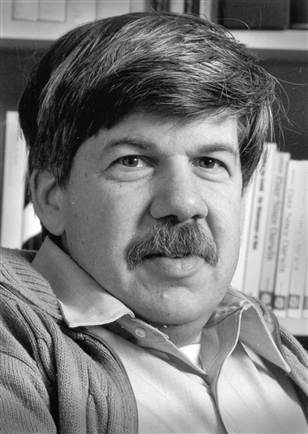
\includegraphics[width=\textwidth]{../figs/Gould.jpg}};
\end{tikzpicture}
\end{columns}
\vhalf
\lfr{Image: Harvard University  /  AP }
\end{frame}

%=====

% Main slides
\begin{ftst}
{Statistical Intervals}
{Introduction}
Statistical intervals are important in quantifying the uncertainty associated to a given estimate;
\vone
As an example, let's recap the coaxial cables example: \textit{a coaxial cable manufacturing operation produces cables with a target resistance of $50\Omega$ and a standard deviation of $2\Omega$. Assume that the resistance values can be well modeled by a normal distribution}.
\vone
Let us now suppose that a sample mean of $N=25$ observations of resistance  yields $\bar{x} = 48$. Given the sampling variability, it is very likely that this value is not exactly the true value of $\mu$, but we are so far unable quantify how much uncertainty there is in this estimate.
\end{ftst}

%=====

\begin{ftst}
{Statistical Intervals}
{Definition}
\textit{Statistical intervals} define regions that are likely to contain the true value of an estimated parameter. 
\vone
More formally, it is generally possible to quantify the level of uncertainty associated with the estimation, thereby allowing the derivation of sound conclusions at predefined levels of certainty.
\vone
Three of the most common types of interval are:

\bitems Confidence intervals;
	\spitem Tolerance intervals;
	\spitem Prediction intervals;
\eitem
\end{ftst}

%=====

\begin{ftst}
{Confidence Intervals}
{Definition}
Confidence intervals quantify the degree of uncertainty associated with the estimation of population parameters such as the mean or the variance.
\vone
Can be defined as ``\textit{the interval that contains the true value of a given population parameter with a confidence level of $100(1-\alpha)$}'';

\bitems \textbf{Wrong}: ``there is a $95\%$ chance that the interval contains the true population mean.''
\spitem \textbf{right}: ``The method used to derive the interval has a hit rate of $95\%$'' - i.e., the interval generated has a $95\%$ chance of ``capturing'' the true population parameter.
\eitem

Easier to understand if you think about the confidence level as a confidence in the \textbf{method}, not in the interval.
\end{ftst}

%=====

\begin{ftst}
{Confidence Intervals}
{Example: 100 $CI_{.95}$ for a sample of 25 observations}
\centering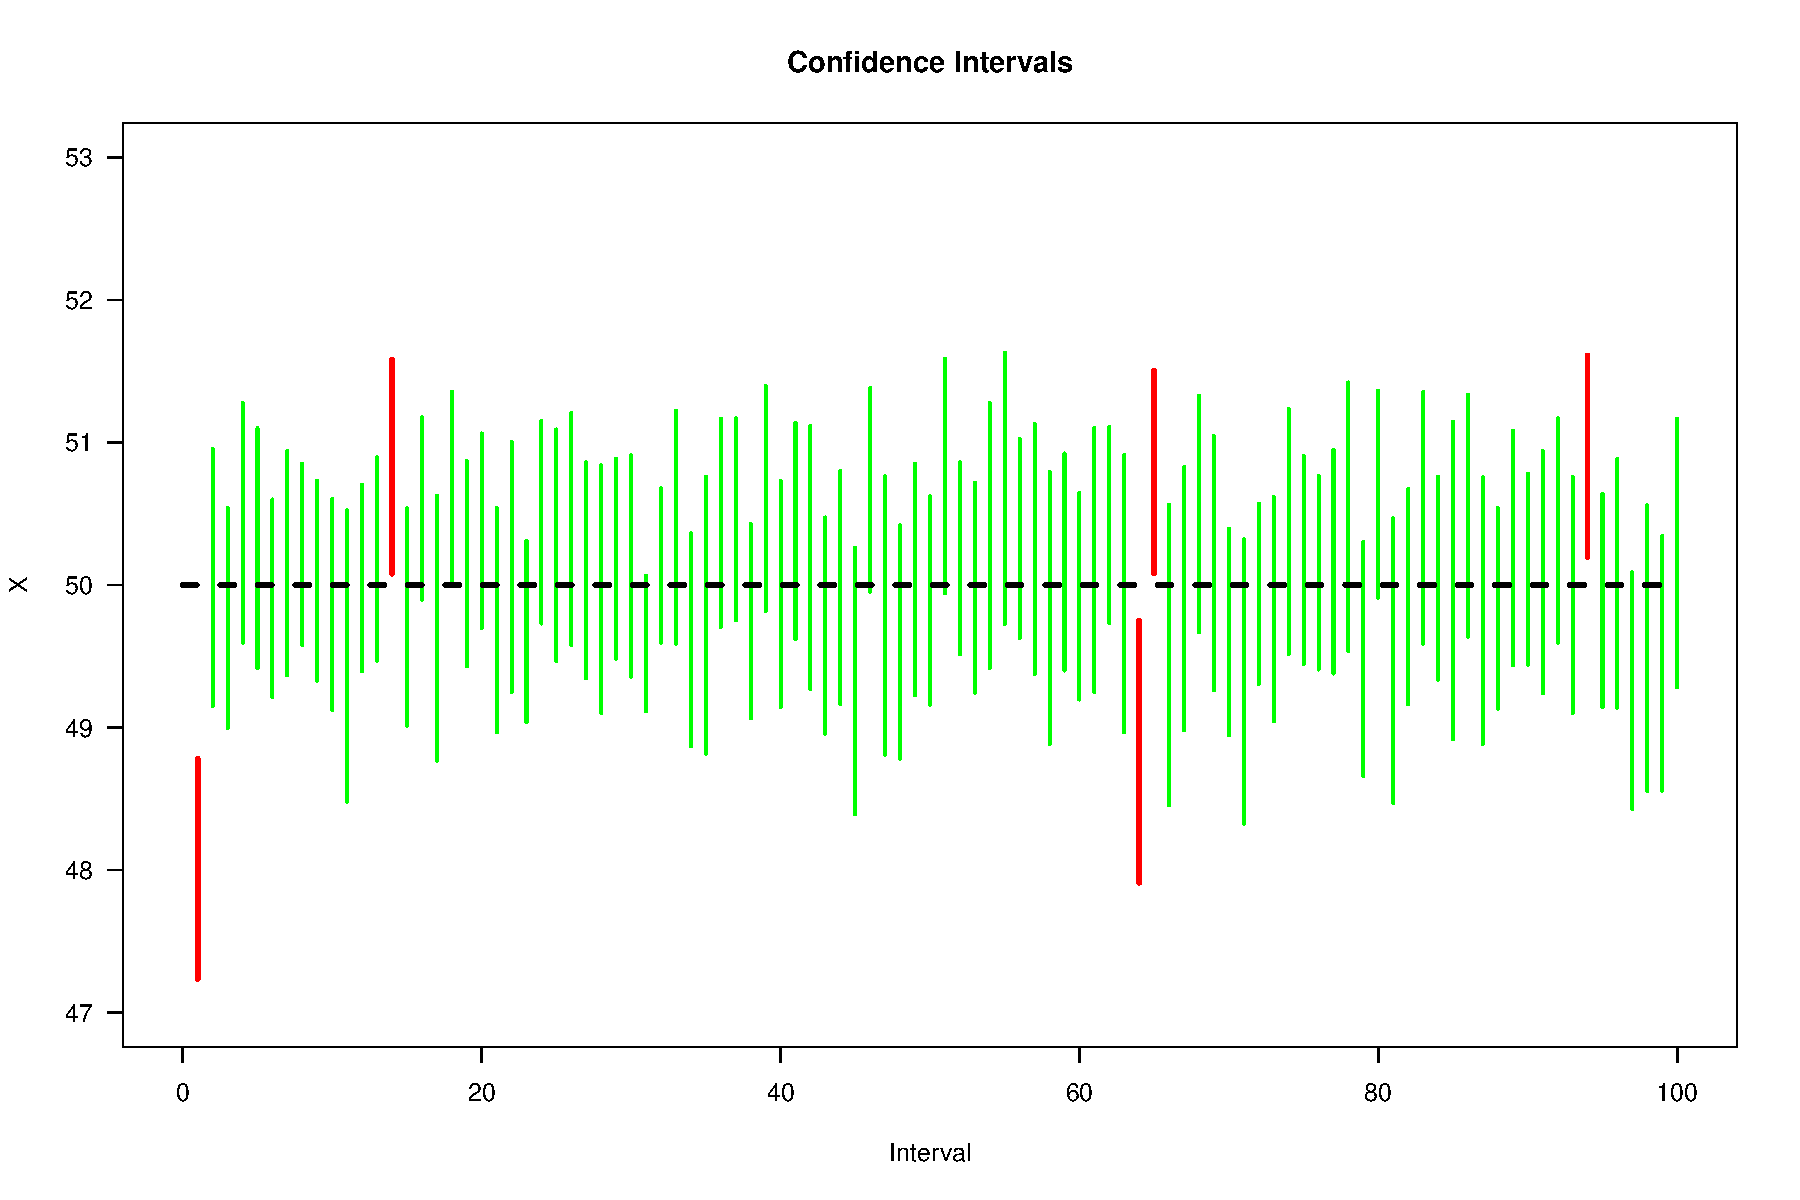
\includegraphics[width=.9\textwidth]{../figs/CIs.pdf}
\lfr{For an interactive demonstration of the factors involved in the definition of a confidence interval, see \url{http://orcslab.cpdee.ufmg.br:3838/CI/}}
\end{ftst}

%=====

\begin{ftst}
{Confidence Intervals}
{CI on the Mean of a Normal Variable}
The two-sided $CI_{(1-\alpha)}$ for the mean of a normal population with known variance $\sigma^2$ is given by:
\beqs
\bar{x}+\frac{\sigma}{\sqrt{N}}z_{(\alpha/2)}\leq\mu\leq\bar{x}+\frac{\sigma}{\sqrt{N}}z_{(1-\alpha/2)}
\eqs
\noindent where $(1-\alpha)$ is the confidence level and $z_{(x)}$ is the $x$-quantile of the standard normal distribution.
\vone
For the more usual case with an unknown variance,
\beqs
\bar{x}+\frac{s}{\sqrt{N}}t_{(\alpha/2;N-1)}\leq\mu\leq\bar{x}+\frac{s}{\sqrt{N}}t_{(1-\alpha/2;N-1)}
\eqs
\noindent where $t_{(x;N-1)}$ is the $x$-quantile of the t distribution with $N-1$ degrees of freedom.
\end{ftst}

%=====

\begin{ftst}
{Confidence Intervals}
{CI on the Variance of a Normal Variable}
Similarly, a two-sided confidence interval on the variance of a normal variable can be easily calculated:
\beqs
\frac{(N-1)s^2}{\chi^2_{\alpha/2;N-1}}\leq\sigma^2\leq\frac{(N-1)s^2}{\chi^2_{1-\alpha/2;N-1}}
\eqs
\noindent where $\chi^2_{\alpha/2;N-1}$ and $\chi^2_{1-\alpha/2;N-1}$ are the upper and lower $(\alpha/2)$-quantiles of the $\chi^2$ distribution with $N-1$ degrees of freedom, respectively.
\end{ftst}

%=====

\begin{ftst}
{Tolerance Intervals}
{Definition}
``\textit{A tolerance interval is an \textbf{enclosure} interval for a specified proportion of the sampled population, not its mean or standard deviation. For a specified confidence level, you may want to determine lower and upper bounds such that a given percent of
the population is contained within them.}''$^{[1]}$.

\centering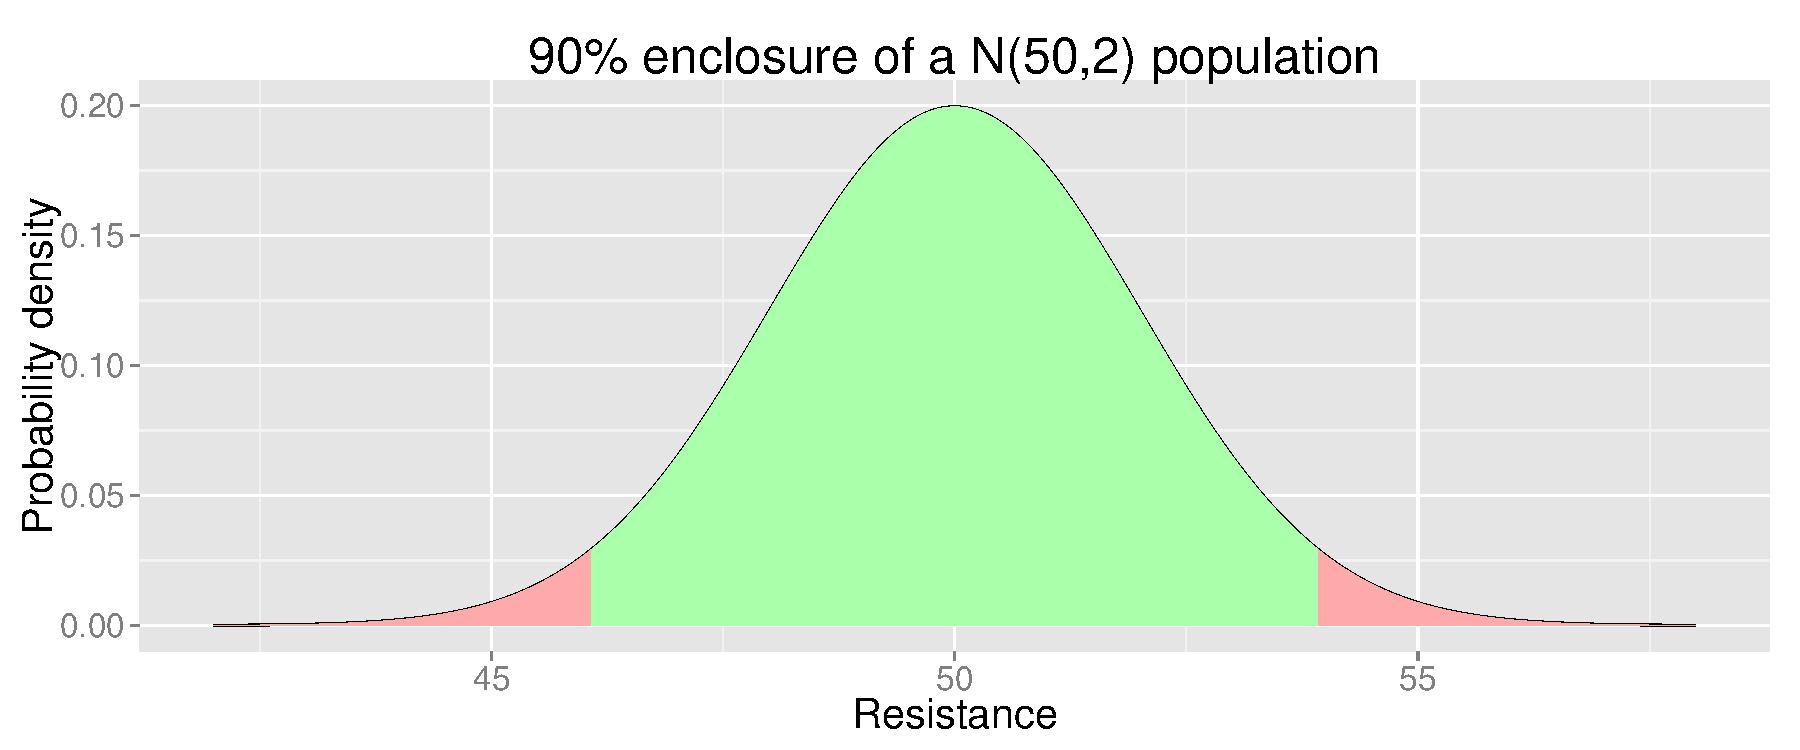
\includegraphics[width=\textwidth]{../figs/enclosure.pdf}
\lfr{[1] J.G. Ram\'irez: \url{http://goo.gl/NJz7ot}}
\end{ftst}

%=====

\begin{ftst}
{Tolerance Intervals}
{Definition}
The common practice in engineering of defining specification limits by adding $\pm3\sigma$ to a given estimate of the mean arises from this definition - for a normally-distributed population, aproximately $99.75\%$ of the observations will fall within these limits.
\vone
However, as in most cases the true population variance is unknown, one has to use its estimate $s^2$ and compensate for the uncertainty in this estimation. The two-sided tolerance interval is then given as:

\beqs
\bar{x}\pm \sqrt{\frac{\left(N-1\right)\left(N+z_{(\alpha/2)}^{2}\right)}{N\ \chi^2_{(\gamma;N-1)}}} 
\eqs
\vhalf
\noindent wherein $\gamma$ is the proportion of the population to be enclosed, and $1-\alpha$ represents the desired confidence level for the interval.
\end{ftst}

%=====

\begin{ftst}
{Prediction Intervals}
{Definition}
Prediction intervals quantify the uncertainty associated with forecasting the value of a future observation;
\vone
Essentially, one is interested in obtaining an interval within which he or she can declare that the next observation will fall with a given probability;
\vone
For a normal distribution, we have:

\beqs
\bar{x} +  t_{(\alpha/2;N-1)}s\sqrt{1+\frac{1}{N}}\leq X_{N+1}\leq\bar{x} + t_{(1-\alpha/2;N-1)}s\sqrt{1+\frac{1}{N}}
\eqs
\vhalf
\noindent which is similar to the confidence interval for the mean, but adding 1 to the term within the square root to account for the prediction noise.
\end{ftst}

%=====

\begin{ftst}
{Statistical Intervals}
{Wrapping up}
Statistical intervals quantify the uncertainty associated with different aspects of estimation;
\vone
Reporting intervals is always better that point estimates, as it provides to you (and your readers) the necessary information to quantify the location and spread of your estimated values;
\vone
The correct interpretation is a little tricky (although not that difficult)$^{[2]}$, but it is essential in order to derive the correct conclusions based on the statistical interval of interest.
\lfr{[2] See the table at the end of: \url{http://goo.gl/NJz7ot}}
\end{ftst}

%=====


\begin{ftst}
{Bibliography}
{\ }
\scriptsize
\textbf{Required reading}

\benums J.G. Ram\'irez, \textit{Statistical Intervals: Confidence, Prediction, Enclosure}: \url{http://goo.gl/NJz7ot}
\item D.C. Montgomery and G.C. Runger, \textit{Applied Statistics and Probability for Engineers}, Chapter 8. 3rd Ed., Wiley 2005.
\eenum

\textbf{Recommended reading}

\benums Simply Statistics (blog) - \url{http://simplystatistics.org}
\item R. Dawkins, \textit{Climbing Mount Improbable}, W.W.Norton\&Co.,1997.
\eenum
\end{ftst}

%=====

\begin{ftstf}{About this material}{Conditions of use and referencing}
\centering\footnotesize This work is licensed under the Creative Commons CC BY-NC-SA 4.0 license\\(Attribution Non-Commercial Share Alike International License version 4.0).\\
\vhalf
\url{http://creativecommons.org/licenses/by-nc-sa/4.0/}\\
\vone
\footnotesize Please reference this work as:\\
\footnotesize \flushleft Felipe Campelo (2015), \textit{Lecture Notes on Design and Analysis of Experiments}.\\Online: {\scriptsize\url{https://github.com/fcampelo/Design-and-Analysis-of-Experiments}}\\
Version 2.11, Chapter 4; Creative Commons BY-NC-SA 4.0.\\

\begin{Verbatim}[fontsize=\tiny]
    @Misc{Campelo2015-01,
      title={Lecture Notes on Design and Analysis of Experiments},
      author={Felipe Campelo},
      howPublished={\url{https://github.com/fcampelo/Design-and-Analysis-of-Experiments}},
      year={2015},
      note={Version 2.11, Chapter 4; Creative Commons BY-NC-SA 4.0.},
    }
\end{Verbatim}

\begin{tikzpicture} [remember picture,overlay]
\node[anchor=south,yshift=0pt] at (current page.south){ \includegraphics[width=.2\textwidth]{../figs/CCSomerights.png}};
\end{tikzpicture}
\end{ftstf}


\end{document}